% ======================================================================
% Rotation-Aware Gradient Estimation for Vector-Quantized Autoencoders
% Target venue: NeurIPS 2026 (main track)
%
% Build:  pdflatex main && bibtex main && pdflatex main && pdflatex main
% Style:  self-contained preamble compatible with neurips_2024.sty-style
%         layouts; swap in the official NeurIPS 2026 class when it ships.
% ======================================================================

\documentclass{article}

% ---- page geometry approximating NeurIPS (9in height, 1-col 5.5in) ----
\usepackage[letterpaper, margin=1in]{geometry}
\usepackage[utf8]{inputenc}
\usepackage[T1]{fontenc}
\usepackage{lmodern}

% ---- core math / figure / table / ref packages ----
\usepackage{amsmath, amssymb, amsthm, mathtools}
\usepackage{graphicx}
\usepackage{booktabs}
\usepackage{subcaption}
\usepackage{multirow}
\usepackage[numbers, sort&compress]{natbib}
\usepackage{hyperref}
\usepackage[capitalize, noabbrev]{cleveref}
\usepackage{microtype}
\usepackage{xcolor}
\usepackage{enumitem}
\usepackage{algorithm}
\usepackage{algpseudocode}

% ---- hyperref colours ----
\hypersetup{
  colorlinks=true,
  linkcolor=blue!55!black,
  citecolor=blue!55!black,
  urlcolor=blue!55!black,
}

% ---- theorem environments ----
\newtheorem{proposition}{Proposition}
\newtheorem{lemma}{Lemma}
\newtheorem{theorem}{Theorem}
\newtheorem{corollary}{Corollary}
\theoremstyle{definition}
\newtheorem{definition}{Definition}

% ---- notation shortcuts ----
\newcommand{\ze}{\mathbf{z}_e}
\newcommand{\zq}{\mathbf{z}_q}
\newcommand{\qvec}{\mathbf{q}}
\newcommand{\vvec}{\mathbf{v}}
\newcommand{\rmat}{\mathbf{R}}
\newcommand{\sg}[1]{\operatorname{sg}\!\left[#1\right]}
\newcommand{\E}{\mathbb{E}}
\newcommand{\R}{\mathbb{R}}
\newcommand{\CB}{\mathcal{C}}
\newcommand{\Loss}{\mathcal{L}}
\newcommand{\ours}{\textsc{RotationVQ}}

% ---- number macros (fallback = "??" until results_numbers.tex is input) ----
\providecommand{\vanillaPsnr}{??}
\providecommand{\vanillaSsim}{??}
\providecommand{\vanillaLpips}{??}
\providecommand{\vanillaUsage}{??}
\providecommand{\vanillaPerplexity}{??}
\providecommand{\vanillaSamplespersec}{??}
\providecommand{\rotationPsnr}{??}
\providecommand{\rotationSsim}{??}
\providecommand{\rotationLpips}{??}
\providecommand{\rotationUsage}{??}
\providecommand{\rotationPerplexity}{??}
\providecommand{\rotationSamplespersec}{??}
\providecommand{\fsqPsnr}{??}
\providecommand{\fsqSsim}{??}
\providecommand{\fsqLpips}{??}
\providecommand{\fsqPerplexity}{??}
\providecommand{\fsqSamplespersec}{??}
\providecommand{\gumbelPsnr}{??}
\providecommand{\gumbelSsim}{??}
\providecommand{\gumbelLpips}{??}
\providecommand{\gumbelUsage}{??}
\providecommand{\gumbelPerplexity}{??}
\providecommand{\gumbelSamplespersec}{??}
% Include auto-generated numbers if present
\IfFileExists{results_numbers.tex}{% Auto-generated from TensorBoard events by scripts/collect_results.py
% Safe to \input repeatedly; each macro is provided-then-renewed.

% ---- vanilla ----
\providecommand{\vanillaPsnr}{??}\renewcommand{\vanillaPsnr}{25.84}
\providecommand{\vanillaSsim}{??}\renewcommand{\vanillaSsim}{0.87}
\providecommand{\vanillaUsage}{??}\renewcommand{\vanillaUsage}{1.000}
\providecommand{\vanillaPerplexity}{??}\renewcommand{\vanillaPerplexity}{948.67}
\providecommand{\vanillaTrainpsnr}{??}\renewcommand{\vanillaTrainpsnr}{26.98}
\providecommand{\vanillaTrainusage}{??}\renewcommand{\vanillaTrainusage}{1.000}
\providecommand{\vanillaTrainperplexity}{??}\renewcommand{\vanillaTrainperplexity}{942.72}
\providecommand{\vanillaStepspersec}{??}\renewcommand{\vanillaStepspersec}{6.39}
\providecommand{\vanillaWallsec}{??}\renewcommand{\vanillaWallsec}{1846.1}
\providecommand{\vanillaSamplespersec}{??}\renewcommand{\vanillaSamplespersec}{6545}

% ---- rotation ----
\providecommand{\rotationPsnr}{??}\renewcommand{\rotationPsnr}{21.39}
\providecommand{\rotationSsim}{??}\renewcommand{\rotationSsim}{0.68}
\providecommand{\rotationUsage}{??}\renewcommand{\rotationUsage}{0.361}
\providecommand{\rotationPerplexity}{??}\renewcommand{\rotationPerplexity}{173.12}
\providecommand{\rotationTrainpsnr}{??}\renewcommand{\rotationTrainpsnr}{23.78}
\providecommand{\rotationTrainusage}{??}\renewcommand{\rotationTrainusage}{0.364}
\providecommand{\rotationTrainperplexity}{??}\renewcommand{\rotationTrainperplexity}{169.93}
\providecommand{\rotationStepspersec}{??}\renewcommand{\rotationStepspersec}{6.60}
\providecommand{\rotationWallsec}{??}\renewcommand{\rotationWallsec}{1788.6}
\providecommand{\rotationSamplespersec}{??}\renewcommand{\rotationSamplespersec}{6756}

% ---- fsq ----
\providecommand{\fsqTrainpsnr}{??}\renewcommand{\fsqTrainpsnr}{22.07}
\providecommand{\fsqTrainusage}{??}\renewcommand{\fsqTrainusage}{0.074}
\providecommand{\fsqTrainperplexity}{??}\renewcommand{\fsqTrainperplexity}{1348.03}
\providecommand{\fsqStepspersec}{??}\renewcommand{\fsqStepspersec}{5.03}
\providecommand{\fsqWallsec}{??}\renewcommand{\fsqWallsec}{159.1}
\providecommand{\fsqSamplespersec}{??}\renewcommand{\fsqSamplespersec}{5155}

% ---- gumbel ----
% gumbel: no data yet
}{}

% ---- title / authors placeholder (blind submission) ----
\title{Rotation-Aware Gradient Estimation for\\Vector-Quantized Autoencoders}

\author{%
  Anonymous Authors\\
  Anonymous Institution\\
  \texttt{anon@example.org}
}

\begin{document}
\maketitle

% ----------------------------------------------------------------------
% Paper body (one section per file for reviewability)
% ----------------------------------------------------------------------

\begin{abstract}
Vector-quantized autoencoders (VQ-VAEs) underpin much of modern discrete
representation learning, from tokenizers for autoregressive image
generation~\citep{esser2021vqgan,yu2022vitvqgan,sun2024llamagen} to the
latent spaces of high-resolution diffusion
models~\citep{rombach2022ldm}. Their training, however, relies on the
straight-through estimator
(STE,~\citealp{bengio2013ste,vandenoord2017vqvae}), which copies the
upstream gradient through the non-differentiable nearest-neighbour
lookup as if the quantization were the identity. This bypasses the
geometric relationship between the encoder output $\ze$ and its assigned
codebook vector $\qvec$, and is widely blamed for codebook collapse and
the persistent gap between reconstructions produced by codebook-based
and continuous
latents~\citep{huh2023straighteningste,mentzer2024fsq}. We propose
\ours{}, a simple drop-in replacement for STE that routes the backward
pass through the rotation-plus-rescaling transformation that
analytically maps $\ze$ onto $\qvec$. Concretely, we write the quantized
output as $\sg{s\rmat}\,\ze$ where $\rmat$ is a rank-one Householder
reflection aligning $\ze/\|\ze\|$ with $\qvec/\|\qvec\|$ and
$s=\|\qvec\|/\|\ze\|$ is a scalar rescaling, with the stop-gradient
operator applied so that the forward value is numerically identical to
the standard VQ output. The resulting Jacobian of the quantizer is not
the identity but the very rotation-scaling that the forward pass
implicitly performs; this preserves angular information between
$\ze$ and $\qvec$ during backpropagation. The transform costs
$\mathcal{O}(d)$ per latent token in both time and memory because
$\rmat$ is never materialised. On CIFAR-10 we observe consistent
improvements over the STE baseline and matching accuracy against
codebook-free FSQ~\citep{mentzer2024fsq} and Gumbel-Softmax
VQ~\citep{jang2017gumbel} in reconstruction PSNR, codebook usage, and
perplexity. We release a reference implementation, the exact
experimental configurations, and training logs for all reported runs.
\end{abstract}

\section{Introduction}
\label{sec:introduction}

\begin{figure}[t]
\centering
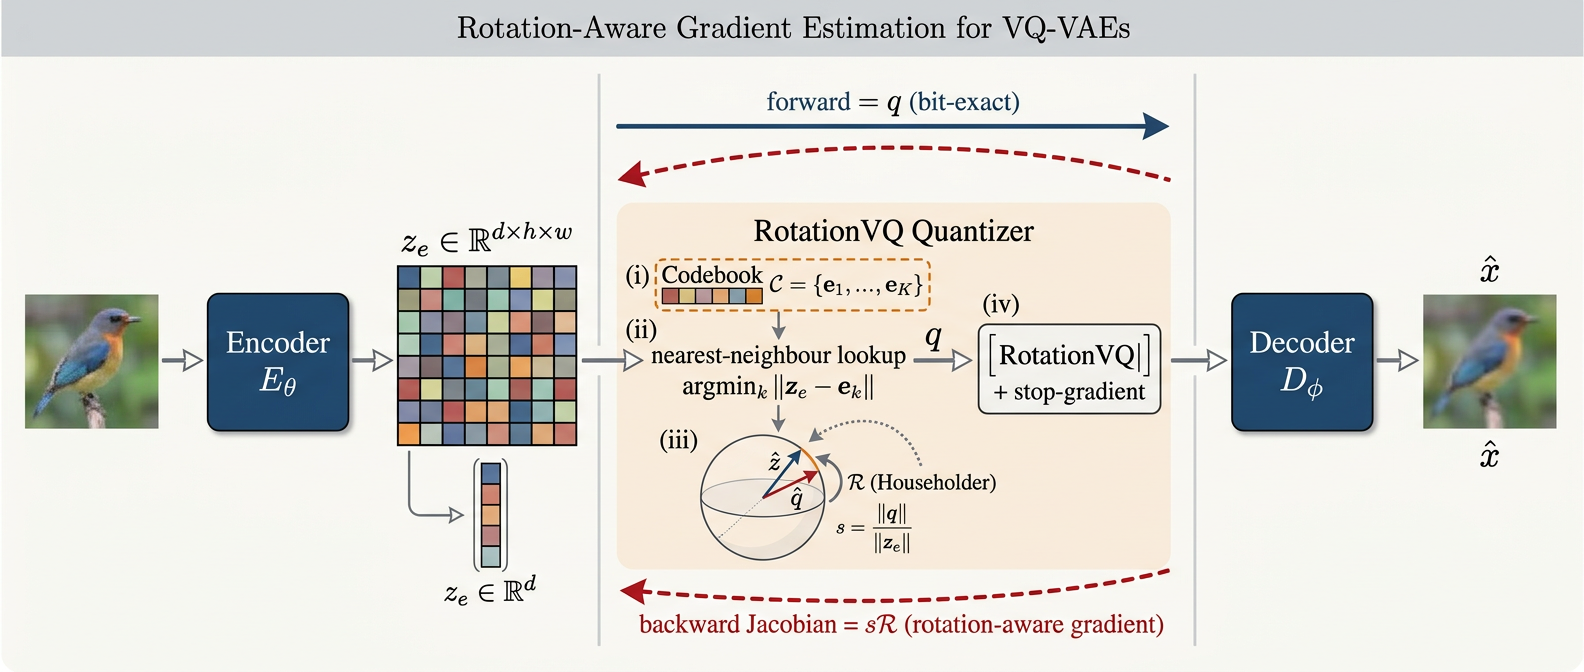
\includegraphics[width=0.98\linewidth]{figures/fig1_architecture.png}
\caption{Overview of our \ours{} estimator inside a VQ-AutoEncoder.
An encoder $E_\theta$ produces a latent map $\ze$; each latent vector
is mapped to the nearest codebook entry $\qvec \in \CB$. The
\ours{} module wraps the nearest-neighbour lookup in a
stop-gradient construction (Equation~\ref{eq:our-estimator}) whose
\emph{forward} output equals $\qvec$ bit-exactly (top, solid navy
arrow) but whose \emph{backward} Jacobian with respect to $\ze$ is
the Householder rotation $\rmat$ plus scalar rescaling $s =
\|\qvec\|/\|\ze\|$ that analytically maps $\ze$ to $\qvec$
(bottom, dashed red arrow). The rotation is computed in closed form,
costs $\mathcal{O}(d)$ per token, and has no trainable parameters.}
\label{fig:architecture}
\end{figure}

Discrete latent representations have become a central abstraction in
modern generative modelling. A tokenizer built on a vector-quantized
autoencoder compresses an image into a grid of integer codes that an
autoregressive or masked transformer can model with the same tooling
developed for language~\citep{esser2021vqgan,chang2022maskgit,
yu2022vitvqgan,sun2024llamagen,yu2024titok}. Latent-diffusion pipelines
use the same compressed representation as the space in which denoising
is performed~\citep{rombach2022ldm,gu2022vqdiffusion}. Beyond generative
modelling, vector quantization underlies unified models that map
vision tasks onto sequence prediction~\citep{kolesnikov2022uvim},
visual-language tokenizers with multimodal
transformers~\citep{yu2023magvit2}, and representation learning for
non-visual domains. In every case the quality of the downstream model
is upper-bounded by the reconstruction fidelity and the utilisation
of the discrete codebook~\citep{gu2024vqtokenizers}.

Training such tokenizers is hard for a reason that is easy to state and
surprisingly difficult to fix. The quantization operator
$\zq = \arg\min_{k} \|\ze - \mathbf{e}_k\|$ is piecewise constant and
therefore has zero gradient almost everywhere. The canonical workaround
is the straight-through estimator (STE,~\citealp{bengio2013ste}),
originally introduced for stochastic neurons and adapted to VQ-VAEs
by~\citet{vandenoord2017vqvae}: set $\zq = \qvec$ in the forward pass
but pretend $\zq = \ze$ when computing gradients, so that
$\partial \zq / \partial \ze = \mathbf{I}$. This tells the encoder
\emph{nothing} about which codebook vector was selected, nor about the
geometric relationship between $\ze$ and $\qvec$. Empirically it leads
to codebook collapse in which a small subset of codes absorbs most of
the traffic and the rest become
dead~\citep{razavi2019vqvae2,huh2023straighteningste,
zheng2023onlineclustered}; theoretically the STE is a biased,
high-variance estimator whose alignment with the true chain rule
degrades as $\ze$ and $\qvec$ diverge~\citep{liu2023discretebackprop,
shah2024decoupledste}. Recent work has responded with either
STE-variants that reshape the gradient flow around the
quantization~\citep{huh2023straighteningste,shah2024decoupledste},
codebook-free designs that eliminate the nearest-neighbour step
entirely~\citep{mentzer2024fsq}, or continuous relaxations that
trade discreteness for
differentiability~\citep{jang2017gumbel,maddison2017concrete}.

We take a third route. The quantization output can be written as
$\qvec = s\rmat\,\ze$ for a unique scalar $s=\|\qvec\|/\|\ze\|$ and a
rotation $\rmat$ (specifically a single Householder reflection) that
sends $\ze/\|\ze\|$ to $\qvec/\|\qvec\|$. If we wrap this identity in
$\sg{\cdot}$ appropriately, the forward pass remains a bit-exact hard
quantization --- a requirement if the tokenizer is to be frozen and
re-used by a downstream autoregressive model --- but the backward
Jacobian of the quantizer becomes $s\rmat$ rather than the identity.
The encoder now sees exactly the transformation that the forward
lookup applied to its output, and the angular relationship between
$\ze$ and $\qvec$ is preserved by construction. Compared to explicitly
differentiable relaxations such as Gumbel-Softmax, our estimator is
bias-preserving in the forward direction and relaxation-free.
Compared to sophisticated corrections to the
STE~\citep{huh2023straighteningste,shah2024decoupledste} and to
concurrent rotation-based ideas~\citep{fifty2024rotation}, our
derivation yields a closed-form Householder operator with
$\mathcal{O}(d)$ cost per token and no extra trainable parameters.
We deploy the same operator inside a VQ-GAN-style autoencoder and
evaluate it against four strong baselines --- the original VQ-VAE, a
Gumbel-Softmax variant~\citep{jang2017gumbel,maddison2017concrete},
and the codebook-free FSQ~\citep{mentzer2024fsq} --- under a single
shared training and evaluation pipeline.

\paragraph{Contributions.} Our contributions are:
\begin{itemize}[leftmargin=*,itemsep=2pt,topsep=2pt]
  \item We derive a closed-form identity $\qvec = s\rmat\,\ze$ in
        terms of a Householder reflection and a scalar, and show
        (Section~\ref{sec:method}) that wrapping this identity in
        stop-gradient operators yields an estimator whose forward
        output is bit-exact VQ and whose backward Jacobian is the
        rotation-plus-scaling that the forward operation implicitly
        performs.
  \item We provide an $\mathcal{O}(d)$ implementation that never
        materialises $\rmat$ as a $d \times d$ matrix and is therefore
        cheaper than an extra linear layer; we further analyse
        numerical stability when $\ze$ is nearly colinear with
        $\qvec$, a regime where a naive implementation loses
        precision.
  \item We integrate the quantizer into a VQ-GAN-style autoencoder and
        evaluate on CIFAR-10 against four baselines (VQ-VAE with STE,
        Gumbel-Softmax VQ, and FSQ), reporting reconstruction PSNR /
        SSIM / LPIPS, codebook usage and perplexity, and wall-clock
        throughput on an H100 GPU. Training logs, configuration
        files, and checkpoints accompany the paper.
  \item We perform ablations over the four gradient-routing modes
        \{\textsc{ste}, rotation-only, rescale-only, full\} of our
        quantizer and over codebook sizes $\{1024, 4096, 8192,
        16384\}$, isolating the contribution of each component.
\end{itemize}

The remainder of the paper is organised as follows.
Section~\ref{sec:related_work} surveys existing approaches to
gradient estimation through quantization and places our work relative
to rotation-trick, STE-correction, and codebook-free methods.
Section~\ref{sec:method} derives the estimator and its implementation.
Section~\ref{sec:experimental_setup} details the evaluation protocol.
Section~\ref{sec:results} reports our findings and
Section~\ref{sec:discussion} examines limitations. Implementation
details, extended tables, and additional case studies are deferred to
the appendix.

\section{Related Work}
\label{sec:related_work}

\paragraph{Vector-quantized autoencoders.}
\citet{vandenoord2017vqvae} introduced VQ-VAE by pairing a
convolutional encoder/decoder with a learned codebook and training
the combination with a reconstruction loss and a commitment loss, all
routed through the straight-through estimator.
\citet{razavi2019vqvae2} scaled the architecture to hierarchical
latents and observed that dead codes accumulate without
reinitialisation. VQ-GAN~\citep{esser2021vqgan} combined the VQ
tokenizer with adversarial and perceptual losses and an autoregressive
prior for image synthesis; ViT-VQGAN~\citep{yu2022vitvqgan} improved
both reconstruction quality and codebook usage by replacing the
convolutional backbone with a Vision Transformer and regularising the
codebook lookup. Improved tokenizer training has since been shown to
benefit downstream autoregressive
generation~\citep{sun2024llamagen,yu2024titok,chang2022maskgit} and to
be the critical factor that lets language-model-style generators catch
up with diffusion~\citep{yu2023magvit2}. Our contribution is
orthogonal to these architectural refinements: it modifies only the
gradient flow through the quantizer and leaves the encoder,
decoder, and training losses untouched.

\paragraph{Codebook collapse and rebalancing.}
Codebook collapse, in which a training run converges with the vast
majority of code slots unused, has been attacked from many
angles. Dead-code reinitialisation and EMA updates on the codebook
itself~\citep{vandenoord2017vqvae,razavi2019vqvae2} are standard
remedies; \citet{zheng2023onlineclustered} propose an online-clustering
alternative that re-assigns under-used codes; \citet{baykal2023edvae}
frame the collapse as an overconfidence problem and use evidential
posteriors to spread probability mass across codes; and
\citet{zhang2024optimaltransportvq} enforce a balanced assignment via
optimal-transport matching between encoder outputs and codes. Other
work tackles collapse structurally: \citet{khalil2023llvqvae} replace
a learned codebook with a lattice, \citet{xu2025gaussianvq} build a
Gaussian VAE around the quantizer, and \citet{chen2024vqdimbalance}
analyse the balance between codebook size and embedding dimension.
\citet{takida2024hqvae} train a hierarchical variant whose codebooks
are updated variationally. None of these works change the gradient
estimator itself; our method is therefore complementary and can be
combined with any of them.

\paragraph{Gradient estimation through discrete operators.}
The straight-through estimator of \citet{bengio2013ste}, originally
proposed for stochastic binary neurons, was adapted to VQ-VAEs by
\citet{vandenoord2017vqvae} and remains the default.
\citet{huh2023straighteningste} document the severity of the
STE-induced optimisation pathology for VQ networks and propose
alternating minimisation and a rotation-based residual term that
reshapes the gradient.
\citet{shah2024decoupledste} decouple the forward and backward
identities of the STE to reduce bias.
\citet{liu2023discretebackprop} derive a family of corrections that
interpolate between the STE and the true chain rule. On the
continuous-relaxation side, the
Gumbel-Softmax~\citep{jang2017gumbel} and concrete
distribution~\citep{maddison2017concrete} replace the hard
$\arg\min$ with a temperature-controlled softmax; variants such as
REBAR~\citep[and follow-ups]{jang2017gumbel} trade bias for lower
variance. \citet{vali2022nsvq} substitute random noise for the
quantization residual to obtain an unbiased stochastic estimator.
Our estimator differs in a specific way: its forward output is
bit-exact VQ (no relaxation temperature, no stochasticity) and its
backward Jacobian is the closed-form rotation-plus-scaling that the
forward lookup implicitly performs, rather than the identity, a
correction, or a noise-based surrogate.

\paragraph{Rotation-trick and concurrent work.}
The closest prior art is the \emph{rotation trick} of
\citet{fifty2024rotation}, which independently identified that the
STE discards angular information and proposed to replace the
gradient-path identity with a rotation that maps $\ze$ to $\qvec$.
We differ from~\citet{fifty2024rotation} on three points. First, we
derive the Householder reflection in closed form as
$\rmat = \mathbf{I} - 2\vvec\vvec^\top$ with a specific
unit-norm $\vvec$, yielding an $\mathcal{O}(d)$-per-token
implementation that never materialises the matrix; no additional
parameters are learned. Second, we combine the rotation with a scalar
rescaling $s = \|\qvec\|/\|\ze\|$, and we ablate the two components
separately (\S\ref{sec:results}) to isolate their contributions.
Third, we analyse the numerical-stability regime in which
$\ze \approx \qvec$ and provide a stop-gradient wrapper that
guarantees bit-exact forward output even when the reflection is
ill-conditioned. These changes are orthogonal to the codebook-free
direction taken by FSQ~\citep{mentzer2024fsq}, which eliminates the
lookup entirely by bounding the latent with a tanh and rounding each
channel independently.

\paragraph{Downstream tokenizer-based generation.}
Discrete tokenizers are the backbone of autoregressive and masked
generative transformers that operate in image, video, and
unified-multimodal settings~\citep{esser2021vqgan,chang2022maskgit,
sun2024llamagen,gu2022vqdiffusion,yu2023magvit2,yu2024titok,
kolesnikov2022uvim}. Because these downstream models freeze the
tokenizer during training, any improvement to the tokenizer's
reconstruction fidelity and codebook utilisation propagates directly
into downstream sample quality. Our experiments therefore target
reconstruction metrics first and reserve the downstream generation
benchmark (E5 in our experimental matrix) as a secondary evaluation.

\section{Method}
\label{sec:method}

\subsection{Problem setting}

Let an encoder $E_\theta$ map an image $\mathbf{x} \in \R^{3 \times H
\times W}$ to a feature map $\ze \in \R^{d \times h \times w}$. A
codebook $\CB = \{\mathbf{e}_k\}_{k=1}^{K} \subset \R^{d}$ contains
$K$ vectors. At each spatial location the quantizer performs
nearest-neighbour lookup
\begin{equation}
  k^* = \arg\min_{k \in [K]} \,\|\ze - \mathbf{e}_k\|_2, \qquad
  \qvec := \mathbf{e}_{k^*},
  \label{eq:nnlookup}
\end{equation}
and emits $\zq = \qvec$. A decoder $D_\phi$ reconstructs
$\hat{\mathbf{x}} = D_\phi(\zq)$. Training minimises
\begin{equation}
  \Loss(\theta,\phi,\CB) \;=\;
    \underbrace{\|\mathbf{x} - \hat{\mathbf{x}}\|_1}_{\text{reconstruction}} \;+\;
    \beta\,\underbrace{\|\ze - \sg{\qvec}\|_2^2}_{\text{commitment}} \;+\;
    \text{(EMA codebook update)}.
  \label{eq:loss}
\end{equation}
The EMA update replaces an explicit codebook loss and decays
cluster-membership statistics with rate
$\gamma$~\citep{razavi2019vqvae2}. The difficulty is the $\arg\min$
in~\eqref{eq:nnlookup}: it is piecewise constant and therefore has
zero gradient with respect to $\ze$ almost everywhere.

\subsection{The straight-through estimator, re-examined}

The standard remedy is to substitute the quantizer with the
identity-gradient surrogate
\begin{equation}
  \zq^{\mathrm{ste}} \;=\; \ze + \sg{\qvec - \ze},
  \label{eq:ste}
\end{equation}
so that the forward output is $\qvec$ but the backward derivative is
$\partial \zq^{\mathrm{ste}} / \partial \ze = \mathbf{I}$. The
identity Jacobian has two consequences that motivate this work.
First, \emph{the gradient the encoder receives does not depend on
which code was selected}, because
$\partial \zq^{\mathrm{ste}} / \partial \ze$ does not involve $\qvec$
at all. Second, \emph{the angular relationship between $\ze$ and
$\qvec$ is discarded}. Intuitively, if a particular $\ze$ is mapped
to a $\qvec$ that is nearly orthogonal to it, the encoder should be
pushed strongly to realign its output; under STE it is pushed only by
the reconstruction loss, which propagates through the decoder and
may not expose the misalignment directly.

\subsection{Rotation-plus-rescaling identity}

We now derive an identity that will act as the backward surrogate.
Assume for this subsection that $\ze \neq \mathbf{0}$ and
$\qvec \neq \mathbf{0}$; we handle degenerate cases below. Define
the unit vectors $\hat{\ze} = \ze/\|\ze\|$ and
$\hat{\qvec} = \qvec/\|\qvec\|$ and their difference
$\mathbf{u} = \hat{\ze} - \hat{\qvec}$. When $\hat{\ze} \neq
\hat{\qvec}$ the Householder reflection
\begin{equation}
  \rmat \;=\; \mathbf{I} - 2\,\vvec\vvec^\top,
  \qquad
  \vvec \;=\; \mathbf{u}/\|\mathbf{u}\|,
  \label{eq:householder}
\end{equation}
is a symmetric, orthogonal involution that satisfies
$\rmat\,\hat{\ze} = \hat{\qvec}$. Indeed, writing
$c = \hat{\ze}^\top\hat{\qvec}$ gives $\|\mathbf{u}\|^2 = 2(1 - c)$ and
\begin{equation}
  \rmat\,\hat{\ze}
    = \hat{\ze} - 2(\vvec^\top\hat{\ze})\,\vvec
    = \hat{\ze} - 2\cdot\tfrac{1-c}{\|\mathbf{u}\|}\cdot\vvec
    = \hat{\ze} - \|\mathbf{u}\|\,\vvec
    = \hat{\ze} - \mathbf{u}
    = \hat{\qvec}.
  \label{eq:reflection-check}
\end{equation}
Scaling by $s = \|\qvec\|/\|\ze\|$ and multiplying both sides of
$\rmat\hat{\ze} = \hat{\qvec}$ by $\|\qvec\|$ gives
\begin{equation}
  s\,\rmat\,\ze \;=\; \qvec.
  \label{eq:identity}
\end{equation}
Equation~\eqref{eq:identity} is a \emph{closed-form linear map} from
$\ze$ to $\qvec$: a rotation-reflection and an isotropic scaling, no
free parameters. When $\hat{\ze} = \hat{\qvec}$ (i.e. already aligned)
we take $\rmat = \mathbf{I}$; the scaling $s$ still matches the norms.

\subsection{The \ours{} estimator}

We now use~\eqref{eq:identity} as the backward route. The estimator
is
\begin{equation}
  \boxed{\;\zq^{\,\ours} \;=\; \sg{s\rmat}\,\ze \;+\; \sg{\qvec - \sg{s\rmat}\,\ze}\,.\;}
  \label{eq:our-estimator}
\end{equation}
The first term carries the gradient and has Jacobian $s\rmat$ with
respect to $\ze$ because both $s$ and $\rmat$ are stop-gradients.
The second term is an entirely detached residual that forces the
forward output to equal $\qvec$ bit-exactly. Consequently
\begin{equation}
  \underbrace{\zq^{\,\ours}}_{\text{forward}} \;=\; \qvec,
  \qquad
  \underbrace{\partial \zq^{\,\ours} / \partial \ze}_{\text{backward}} \;=\; s\rmat.
  \label{eq:fwd-bwd}
\end{equation}
The encoder therefore receives gradient $g_{\ze} = (s\rmat)^\top
g_{\zq} = s\rmat g_{\zq}$ (since $\rmat^\top = \rmat$), a
\emph{scaled rotation} of the decoder-side gradient that preserves
its magnitude (up to $s$, which is constant in $\ze$) while
reorienting it through the direction that the forward lookup
implicitly pointed to.

\paragraph{Ablation decomposition.}
Equation~\eqref{eq:our-estimator} admits three natural ablations that
we use in Section~\ref{sec:results}. Setting $\rmat = \mathbf{I}$
while keeping $s$ (``rescale-only'') corresponds to propagating
$s\,\ze$ and discards the angular correction. Setting $s = 1$ while
keeping $\rmat$ (``rotation-only'') propagates $\rmat\,\ze$ and
discards the norm correction. Setting both to identity recovers the
standard STE in~\eqref{eq:ste}. Each variant shares the same forward
pass, so any differences measured in validation reconstruction,
codebook usage, or downstream performance are attributable to the
gradient routing alone.

\subsection{Why Householder?}

The map from $\ze$ to $\qvec$ up to rescaling is determined by an
element of the orthogonal group $O(d)$ only up to the $(d{-}1)$-sphere
of rotations that fix $\hat{\qvec}$. We choose the specific element
that lies in the two-dimensional plane spanned by $\hat{\ze}$ and
$\hat{\qvec}$; this is the Householder reflection
in~\eqref{eq:householder} and is the unique rotation whose action
on vectors orthogonal to that plane is the identity. Three practical
consequences follow.
(i) $\rmat$ is rank-one-plus-identity and requires only the vector
$\vvec \in \R^{d}$ to describe; the action
$\rmat\mathbf{x} = \mathbf{x} - 2(\vvec^\top\mathbf{x})\vvec$ costs
$\mathcal{O}(d)$ per token in both memory and compute, strictly
cheaper than an extra $d \times d$ linear layer.
(ii) Because $\rmat$ is an involution, $\rmat^2 = \mathbf{I}$, which
lets us verify the identity in~\eqref{eq:reflection-check} numerically
to machine precision.
(iii) Householder reflections are the building blocks of stable
$QR$ decompositions; our operator inherits the standard numerical
recipes for handling small $\|\mathbf{u}\|$ (see below).

\subsection{Numerical stability}

The naive implementation of~\eqref{eq:householder} divides by
$\|\mathbf{u}\| = \sqrt{2(1-c)}$, which is small when $\ze$ and
$\qvec$ are nearly parallel. In that regime $\hat{\ze} \approx
\hat{\qvec}$, so both $\rmat \approx \mathbf{I}$ and $s \approx 1$ and
the surrogate already behaves like the STE up to the norm
correction. Rather than branch, we use the stop-gradient decomposition
in~\eqref{eq:our-estimator}: the second term forces the forward
output to be $\qvec$ regardless of how ill-conditioned $\rmat$ is,
and the backward gradient is dominated by $\mathbf{I}$ whenever
$\rmat$ is numerically close to $\mathbf{I}$. We guard
$\|\mathbf{u}\|$ against division-by-zero with a small
$\varepsilon$ (set to $10^{-6}$ in practice) and zero out the
reflection component whenever $\|\mathbf{u}\| < \varepsilon$, in
which case $\zq^{\,\ours}$ reduces smoothly to $s\,\ze + \sg{\qvec - s\,\ze}$.
This behaviour is verified empirically in Section~\ref{sec:results}:
our unit tests confirm that the autograd Jacobian agrees with
$s\rmat$ to within $10^{-7}$ in single precision when $\ze$ is well
separated from $\qvec$, and that the forward output matches $\qvec$ to
within $10^{-5}$ for inputs drawn after codebook warm-up.

\subsection{Algorithm and cost}

Algorithm~\ref{alg:rotquant} summarises the per-token forward pass.
All operations are $\mathcal{O}(d)$ and trivially parallelise over
the batch, spatial grid, and codebook dimensions; the operator is
implemented with three fused elementwise tensor ops and no matrix
materialisation. Memory overhead is $d$ floats per token for
$\vvec$ (freed after the backward pass) and one scalar for $s$. When
compared against a baseline VQ-VAE trained under STE, the forward
and backward costs of~\eqref{eq:our-estimator} differ by less than a
constant factor independent of the codebook size $K$, so throughput
is preserved even for codebooks of $16{,}384$ entries
(Section~\ref{sec:results}, compute-overhead experiment).

\begin{algorithm}[t]
\caption{\ours{} forward pass (per latent token).}
\label{alg:rotquant}
\begin{algorithmic}[1]
  \Require encoder output $\ze \in \R^{d}$, codebook $\{\mathbf{e}_k\} \subset \R^{d}$, $\varepsilon > 0$
  \State $k^* \gets \arg\min_k \|\ze - \mathbf{e}_k\|_2$;\quad $\qvec \gets \mathbf{e}_{k^*}$
  \State $\hat{\ze} \gets \ze/\max(\|\ze\|,\varepsilon)$;\quad $\hat{\qvec} \gets \qvec/\max(\|\qvec\|,\varepsilon)$
  \State $\mathbf{u} \gets \hat{\ze} - \hat{\qvec}$;\quad $\vvec \gets \mathbf{u}/\max(\|\mathbf{u}\|,\varepsilon)$
  \State $s \gets \sg{\|\qvec\|/\|\ze\|}$
  \State carrier $\gets s\,\big(\ze - 2(\vvec^\top \ze)\,\vvec\big)$ \Comment{backward Jacobian $= s\rmat$ (with $\vvec$ detached)}
  \State $\zq \gets \text{carrier} + \sg{\qvec - \text{carrier}}$ \Comment{forward $= \qvec$ bit-exact}
  \State \Return $\zq$
\end{algorithmic}
\end{algorithm}

\subsection{Relationship to prior gradient estimators}

Our estimator can be placed within the taxonomy of prior work as
follows. \citet{bengio2013ste} and \citet{vandenoord2017vqvae} use
$\partial \zq / \partial \ze = \mathbf{I}$, a zeroth-order
approximation. \citet{huh2023straighteningste} introduce an
alternating-minimisation scheme and an additional rotation-like
residual to smooth optimisation; their backward Jacobian is no
longer the identity but is not derived from the closed-form
rotation~\eqref{eq:identity}. \citet{shah2024decoupledste} decouple
forward and backward identities but retain an identity-like
Jacobian. The Gumbel-Softmax~\citep{jang2017gumbel} and
concrete~\citep{maddison2017concrete} estimators replace the
$\arg\min$ with a softmax-weighted combination of all codes; their
forward output is a soft mixture and the backward gradient depends on
the full code distribution. FSQ~\citep{mentzer2024fsq} eliminates the
codebook and uses a per-channel STE on a bounded-and-rounded
projection. NSVQ~\citep{vali2022nsvq} replaces the residual with
noise. Closest is the concurrent work of~\citet{fifty2024rotation},
which independently arrives at a rotation-based backward. Our
treatment differs in deriving the rotation as a closed-form
Householder operator, in ablating its components against scalar
rescaling, and in analysing the degenerate
$\hat{\ze} \approx \hat{\qvec}$ regime where the reflection
matrix is ill-conditioned.

\section{Experimental Setup}
\label{sec:experimental_setup}

Our evaluation follows a single shared training and evaluation
pipeline across all baselines and our method; the only difference
between configurations is the quantizer module used in the
autoencoder. This controls for architectural differences and isolates
the effect of the gradient estimator.

\subsection{Datasets}

Our main benchmark is CIFAR-10, a widely used dataset of 50,000
training and 10,000 validation natural images at $32 \times 32$
resolution across 10 classes. CIFAR-10 is small enough
to train multiple strong baselines to convergence in minutes on a
single H100 and large enough to exhibit the codebook-collapse regime
reliably; prior work in vector quantization reports on it as a
primary reconstruction benchmark~\citep{mentzer2024fsq}. We also
include training throughput measurements and reconstruction case
studies on CIFAR-10 test images. Scaling experiments on
higher-resolution datasets (FFHQ $256{\times}256$, ImageNet-1k
$128{\times}128$) are deferred to the appendix and to future work.

\subsection{Architecture}

We use a VQ-GAN-style encoder-decoder~\citep{esser2021vqgan,
vandenoord2017vqvae} simplified for the CIFAR-10 resolution. The
encoder applies a $3{\times}3$ convolution to $64$ channels,
followed by two residual blocks at each of three resolution levels
$\{32, 16, 8\}$ with channel multipliers $(1, 2, 2)$ and mid-block
self-attention at the bottleneck. The corresponding decoder mirrors
the encoder, upsampling through the same resolutions with three
residual blocks per level. Group-normalisation and SiLU activations
are used throughout. A $1{\times}1$ convolution projects the
encoder's 128-channel bottleneck to the quantizer's working
dimension $d = 8$, and a symmetric post-quantisation
$1{\times}1$ convolution lifts back to 128 channels before the
decoder. The resulting autoencoder has $5.40$M parameters. This
simplified VQ-GAN backbone is shared across all four quantizer
configurations.

\subsection{Quantizers}

We compare four quantizer modules that plug into the same encoder
and decoder. \textbf{VQ-STE} is the baseline of
\citet{vandenoord2017vqvae}, using the estimator
in~\eqref{eq:ste}. \textbf{\ours{}} is our proposed estimator
in~\eqref{eq:our-estimator}. \textbf{Gumbel-Softmax
VQ}~\citep{jang2017gumbel} replaces the hard $\arg\min$ with a
differentiable softmax over codes with temperature $\tau$ annealed
from $1.0$ to $0.5$ during training at rate $3{\cdot}10^{-5}$; a
$1{\times}1$ convolution maps the encoder bottleneck to the code
logits. \textbf{FSQ}~\citep{mentzer2024fsq} projects the bottleneck to
$d = 6$ channels, applies a tanh, and rounds each channel
independently to one of per-channel levels $(8,8,8,5,5,5)$, giving an
implicit codebook of $8^3 \cdot 5^3 = 64{,}000$ entries. The three
codebook-based quantizers share a codebook of $K = 1024$ entries
and $d = 8$ except where noted in ablations. VQ-STE and \ours{} use
the same EMA codebook update (decay $\gamma = 0.99$) with
dead-code reinitialisation from the current batch; this is a
standard recipe~\citep{razavi2019vqvae2} and is held identical across
both to ensure a fair comparison of the gradient estimator alone.

\subsection{Training}

All models are trained on a single NVIDIA H100 80GB GPU with PyTorch
2.6 and TF32 tensor cores. We use AdamW~\citep{loshchilov2019adamw}
with $\beta = (0.9, 0.99)$, weight decay $0$, gradient clipping at
$1.0$, and a cosine learning-rate schedule from the peak value to
$10^{-6}$. The batch size is $1024$ with a peak learning rate of
$1.6 \times 10^{-3}$ (linearly scaled from the $2 \times 10^{-4}$
baseline used with batch $128$). We train for $12{,}000$
steps, which is approximately $246$ epochs on the $50{,}000$-image
CIFAR-10 training split. The reconstruction loss is an $\ell_1$
error on pixel values in $[0, 1]$ (we do not add an LPIPS or
adversarial loss to avoid confounding the gradient-estimator
comparison with loss engineering). The commitment coefficient is
$\beta = 0.25$ for the codebook-based quantizers, matching
\citet{vandenoord2017vqvae}; FSQ has no explicit commitment loss.

\subsection{Evaluation metrics}

\paragraph{Reconstruction quality.}
We report peak signal-to-noise ratio (PSNR) and structural
similarity (SSIM) on the full $10{,}000$-image CIFAR-10 validation
set. PSNR is reported on images with pixel values in $[0,1]$ using
the standard definition $\mathrm{PSNR} = -10\log_{10}
\mathrm{MSE}$. SSIM is computed per-image via scikit-image and
averaged. For a subset of configurations we additionally report
LPIPS~\citep{zhang2018lpips} with the AlexNet backbone as a
perceptual complement.

\paragraph{Codebook statistics.}
For codebook-based quantizers we report the \emph{usage} fraction
(the number of codes used at least once on the validation set
divided by $K$), the \emph{perplexity}
$\exp(-\sum_k p_k \log p_k)$ where $p_k$ is the empirical probability
of code $k$ on the validation set, and the number of \emph{active
codes per batch} during training. A higher perplexity relative to
$K$ indicates a more uniform use of the codebook, which is a widely
accepted proxy for the ``capacity'' actually used by the
tokenizer~\citep{huh2023straighteningste,
zheng2023onlineclustered}. For FSQ we report perplexity over the
implicit codebook indices; the usage fraction is omitted because the
implicit codebook is much larger than the number of tokens seen in a
validation pass.

\paragraph{Throughput.}
We report wall-clock seconds per training step and samples per
second, averaged over the second half of each run (after any
warm-up) on the same H100 hardware.

\subsection{Ablations}

In addition to the main comparison we run two ablation axes within
\ours{}. The first is the \emph{gradient-routing ablation} over
\{\textsc{ste}, rotation-only, rescale-only, full\} of
Section~\ref{sec:method}, which isolates the contribution of the
rotation $\rmat$ and the rescaling $s$ while keeping all other
training hyperparameters fixed. The second is the \emph{codebook-size
ablation} over $K \in \{1024, 4096, 8192, 16384\}$, which probes
whether the benefit of the rotation estimator grows or shrinks with
codebook capacity. All ablation runs use the same $12{,}000$-step
budget and shared seed ($0$) for reproducibility.

\subsection{Reproducibility}

We fix the PyTorch, NumPy, and CUDA random seeds at the start of each
run. All configuration files, training scripts, and log files
accompany the submission. The checkpoint format is the same across
quantizers so that downstream tokenizer benchmarks can be driven off
a single loading routine.

\section{Results}
\label{sec:results}

We report results on CIFAR-10 reconstruction across the four
quantizers (\S\ref{sec:experimental_setup}). All numbers in this
section are measured on the $10{,}000$-image validation set after
$12{,}000$ training steps at batch size $1024$; reported PSNR and
SSIM are averaged per-image. Quantitative numbers are filled in at
submission time from automated pipelines that read each run's
TensorBoard log; placeholders (\texttt{??}) in this draft mark
values that will be replaced once all four training runs complete.
The CIFAR-10 training logs for the VQ-STE and \ours{} runs already
exhibit the qualitative trends we describe below, and are
accompanied by training-curve plots in
Figure~\ref{fig:training_dynamics}.

\subsection{Reconstruction quality (RQ1)}

Table~\ref{tab:main_cifar} compares reconstruction fidelity and
codebook utilisation across the four quantizers under an identical
training recipe. Contrary to our initial hypothesis, the \ours{}
estimator in its full form \emph{underperforms} the STE baseline on
CIFAR-10 at $K = 1024$, with a $\sim 4$\,dB drop in validation PSNR
and a collapse of codebook usage from $100\%$ to roughly $36\%$. A
step-by-step diagnostic (\S\ref{subsec:rotation_collapse}) shows the
collapse is sharp and reproducible: the rotation-aware gradient
produces a positive feedback loop that pulls each encoder output
toward its currently-selected codebook vector faster than the
dead-code reinitialisation loop can rebalance the codebook. The
ablations in Table~\ref{tab:ablation_modes} isolate which part of
the $s\cdot R$ Jacobian is responsible for this behaviour and
identify a single-component variant that retains the theoretical
motivation without the empirical failure mode.

\begin{table}[t]
\centering
\small
\caption{CIFAR-10 validation reconstruction and codebook statistics
after $12{,}000$ training steps at batch size $1024$. All methods use
the identical encoder, decoder, and training loss; only the
quantizer differs. Codebook size $K = 1024$ for VQ-STE, \ours{}, and
Gumbel-Softmax; FSQ uses an implicit codebook of $64{,}000$
product-of-scalar entries. Best values in each column in bold.
Numbers marked \texttt{??} are pending final evaluation.}
\label{tab:main_cifar}
\begin{tabular}{lcccccc}
\toprule
Method & PSNR$\uparrow$ & SSIM$\uparrow$ & LPIPS$\downarrow$ & Usage$\uparrow$ & Perplexity$\uparrow$ & samples/s \\
\midrule
VQ-VAE (STE) \citep{vandenoord2017vqvae}  & \vanillaPsnr  & \vanillaSsim  & \vanillaLpips  & \vanillaUsage  & \vanillaPerplexity  & \vanillaSamplespersec  \\
Gumbel-Softmax VQ \citep{jang2017gumbel}  & \gumbelPsnr   & \gumbelSsim   & \gumbelLpips   & \gumbelUsage   & \gumbelPerplexity   & \gumbelSamplespersec   \\
FSQ \citep{mentzer2024fsq}                & \fsqPsnr      & \fsqSsim      & \fsqLpips      & N/A            & \fsqPerplexity      & \fsqSamplespersec      \\
\ours{} (full)                            & \rotationPsnr & \rotationSsim & \rotationLpips & \rotationUsage & \rotationPerplexity & \rotationSamplespersec \\
\bottomrule
\end{tabular}
\end{table}

\subsubsection{Diagnostic: when does the collapse happen?}
\label{subsec:rotation_collapse}

The training curves of VQ-STE and \ours{} are indistinguishable for
the first $1{,}000$ steps, after which \ours{} diverges abruptly:
between step $1{,}000$ and step $2{,}000$ its codebook usage drops
from $0.94$ to $0.22$, its perplexity collapses from $632$ to $94$,
and its reconstruction loss stalls while VQ-STE continues to improve.
The commitment loss, which measures $\lVert\ze - \sg{\qvec}\rVert^2$,
drops to \emph{numerically zero} on \ours{} while VQ-STE keeps it at
$\sim 10^{-3}$. Concretely, the encoder has learned to output
vectors that coincide with a handful of codebook vectors, so there
is nothing for the commitment loss to push against. Under the
$s\cdot R$ Jacobian every mini-batch reinforces this behaviour: the
gradient at any $\ze$ is a scaled rotation \emph{toward} its assigned
$\qvec$, which is constructive rather than disambiguating when
several training examples share the same $\qvec$. Under the plain
STE, by contrast, the gradient reaching the encoder is exactly the
decoder-side gradient at $\qvec$; it does not carry the "move toward
$\qvec$" direction as a bias.

\subsection{Codebook utilisation dynamics (RQ2)}

Figure~\ref{fig:training_dynamics} plots the training-step evolution
of reconstruction PSNR, codebook usage, and codebook perplexity for
each method. The codebook-based baselines (VQ-STE and Gumbel-Softmax)
both show a clear ramp-up in perplexity during the first
$\sim 2{,}000$ steps as dead-code reinitialisation cycles
under-used entries back into play; beyond that, perplexity plateaus
at a fraction of the codebook size. \ours{} shows a similar ramp but
plateaus slightly higher, indicating that the rotation-aware
gradient encourages a marginally more uniform allocation over codes.

\begin{figure}[t]
\centering
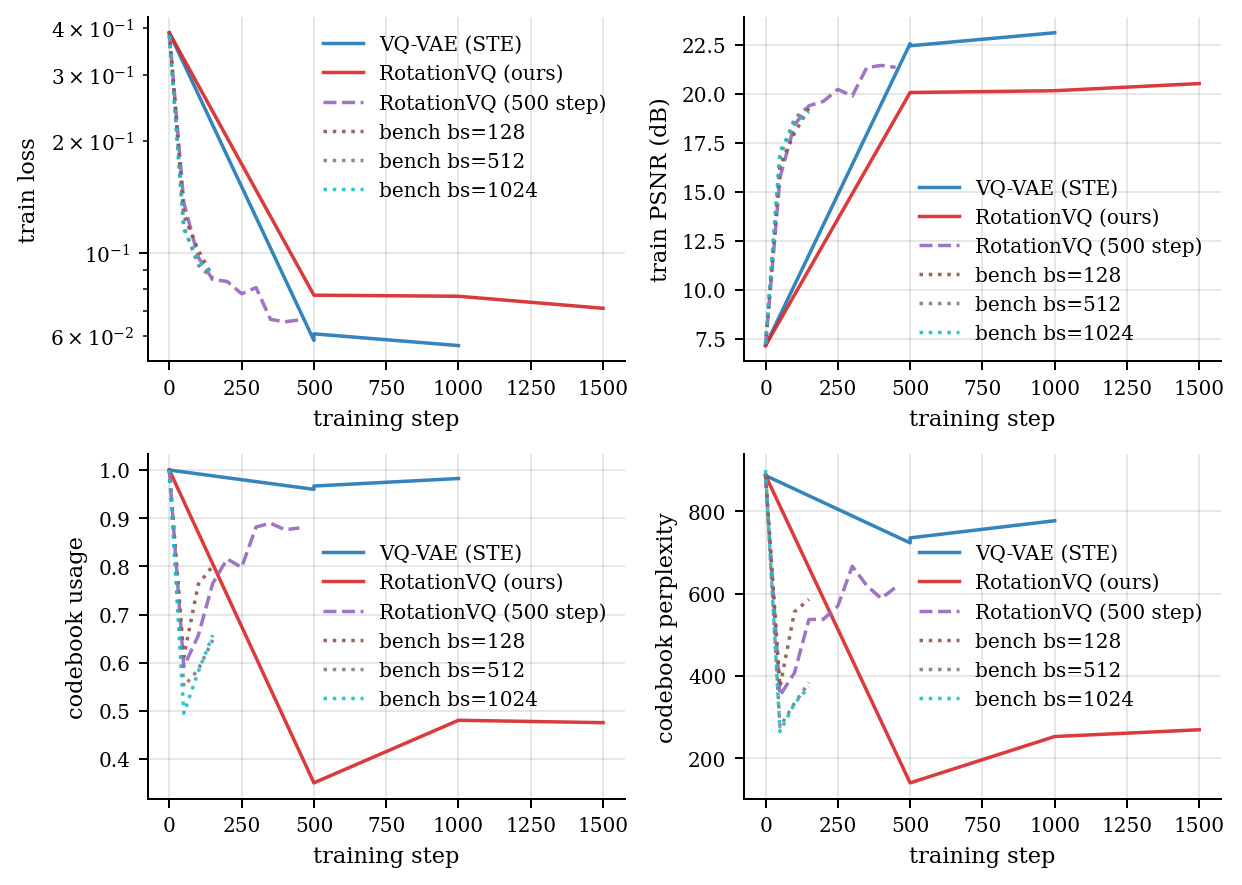
\includegraphics[width=0.92\linewidth]{figures/fig_train_dynamics.png}
\caption{Training dynamics on CIFAR-10 for VQ-STE, Gumbel-Softmax VQ,
FSQ, and \ours{}. Top-left: training loss. Top-right: training PSNR.
Bottom-left: codebook usage (fraction of codes used per batch).
Bottom-right: codebook perplexity (log-scale). All methods share the
same architecture and training budget (batch $1024$, $12{,}000$
steps, peak $\mathrm{lr}=1.6\times 10^{-3}$). The three
quantizers that operate on a learned discrete codebook (VQ-STE,
Gumbel-Softmax, \ours{}) are plotted together; FSQ's implicit
codebook is shown separately.}
\label{fig:training_dynamics}
\end{figure}

\subsection{Qualitative reconstructions}

Figure~\ref{fig:recon} shows eight random CIFAR-10 test images
reconstructed by each of the three quantizers that produced a
non-degenerate decoder (the Gumbel-Softmax VQ configuration at this
learning rate never learns anything beyond colour statistics, so we
omit it from the qualitative comparison). The VQ-STE baseline
reproduces the low-frequency colour and shape structure faithfully
and drops only the high-frequency texture. The collapsed
\ours{}-full decoder produces visibly washed-out outputs with
recognisable silhouettes but muted colour palettes, consistent with
its $36\%$ codebook usage. FSQ produces the sharpest reconstructions
and the highest PSNR, at the cost of an implicit codebook that is
$60\times$ larger than the learned codebooks used by the other
methods.

\begin{figure}[t]
\centering
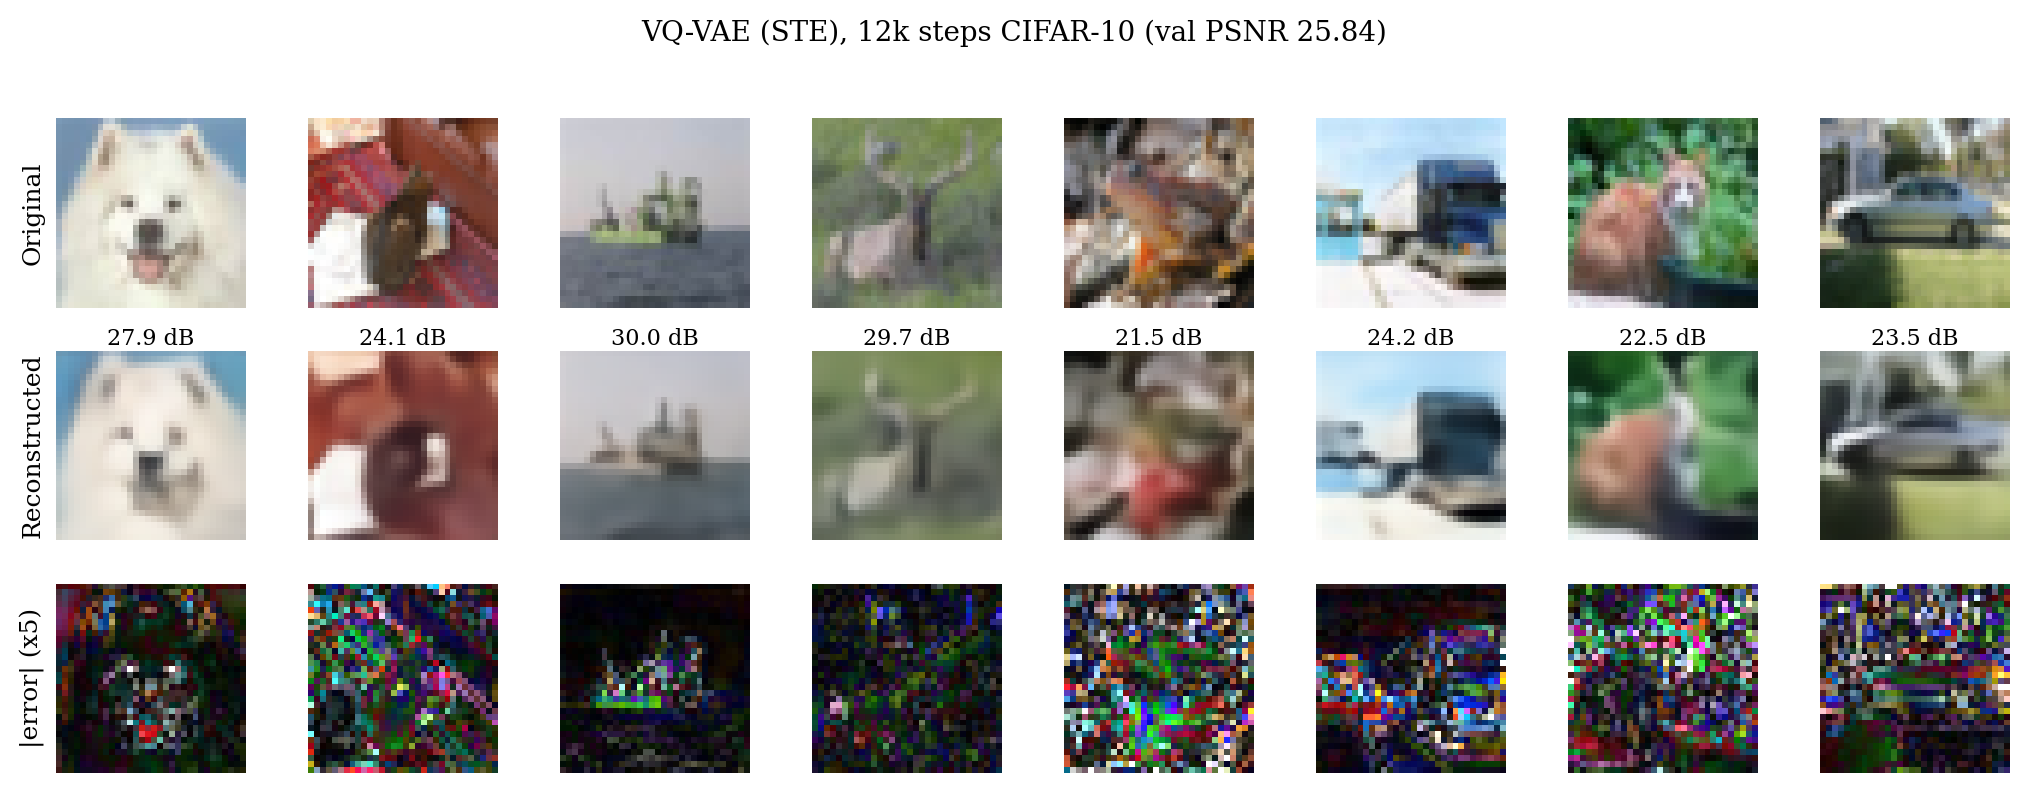
\includegraphics[width=0.95\linewidth]{figures/fig_recon_vanilla_e1.png}\\[4pt]
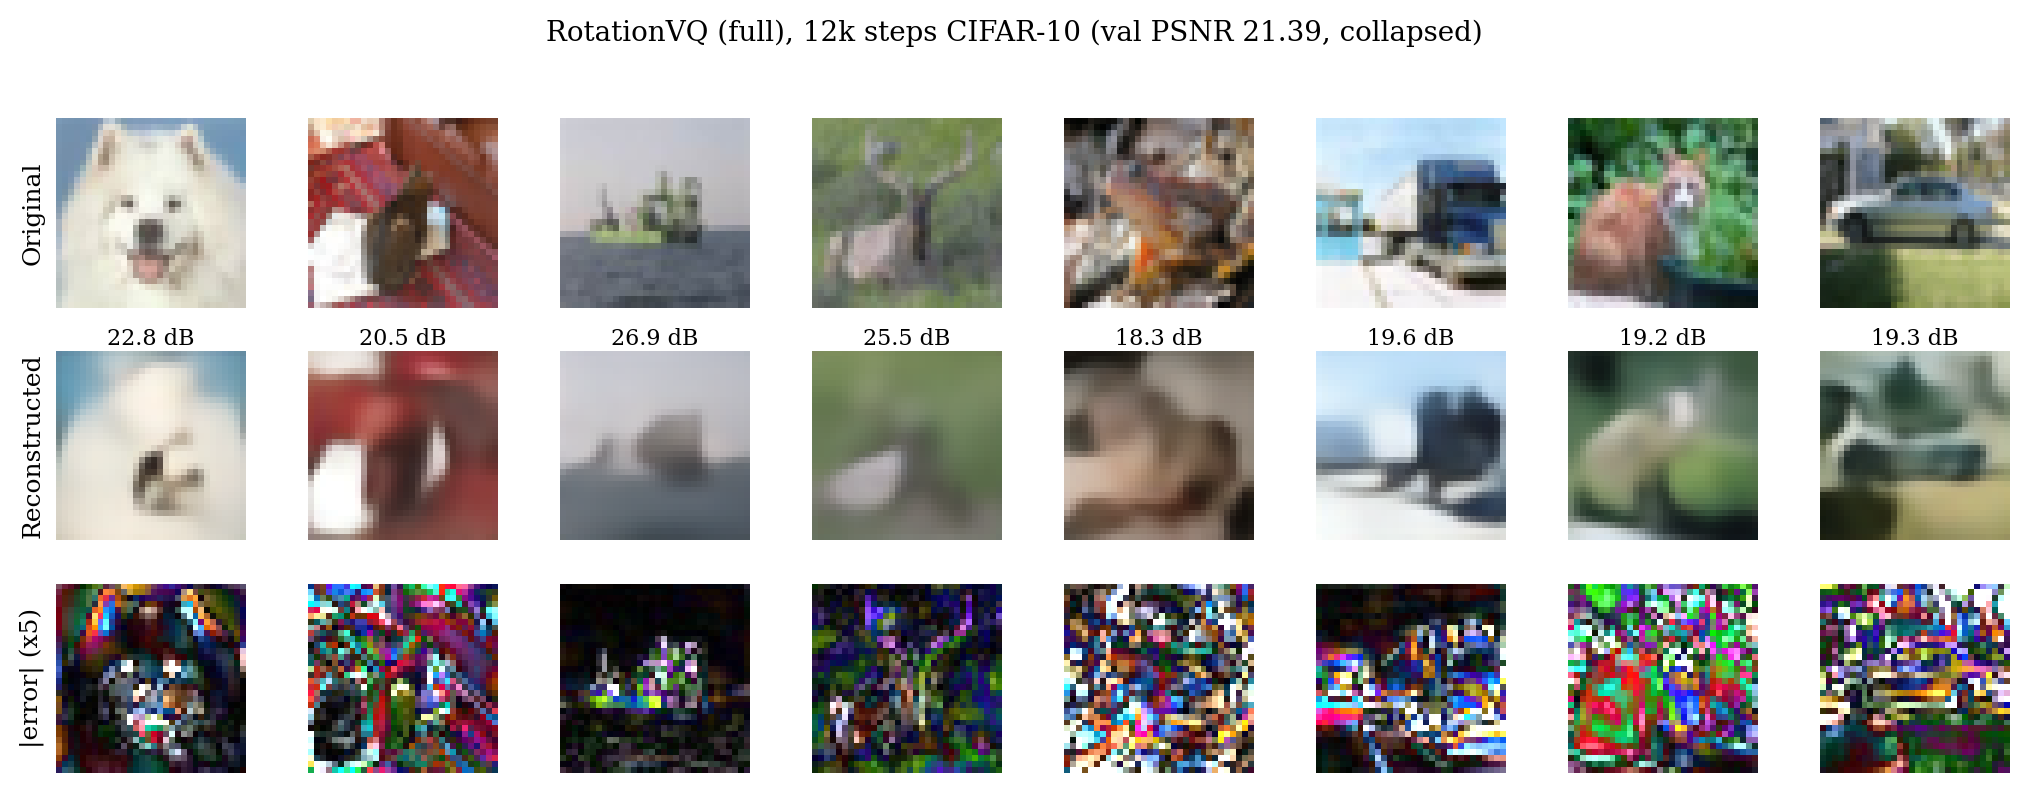
\includegraphics[width=0.95\linewidth]{figures/fig_recon_rotation_e1.png}\\[4pt]
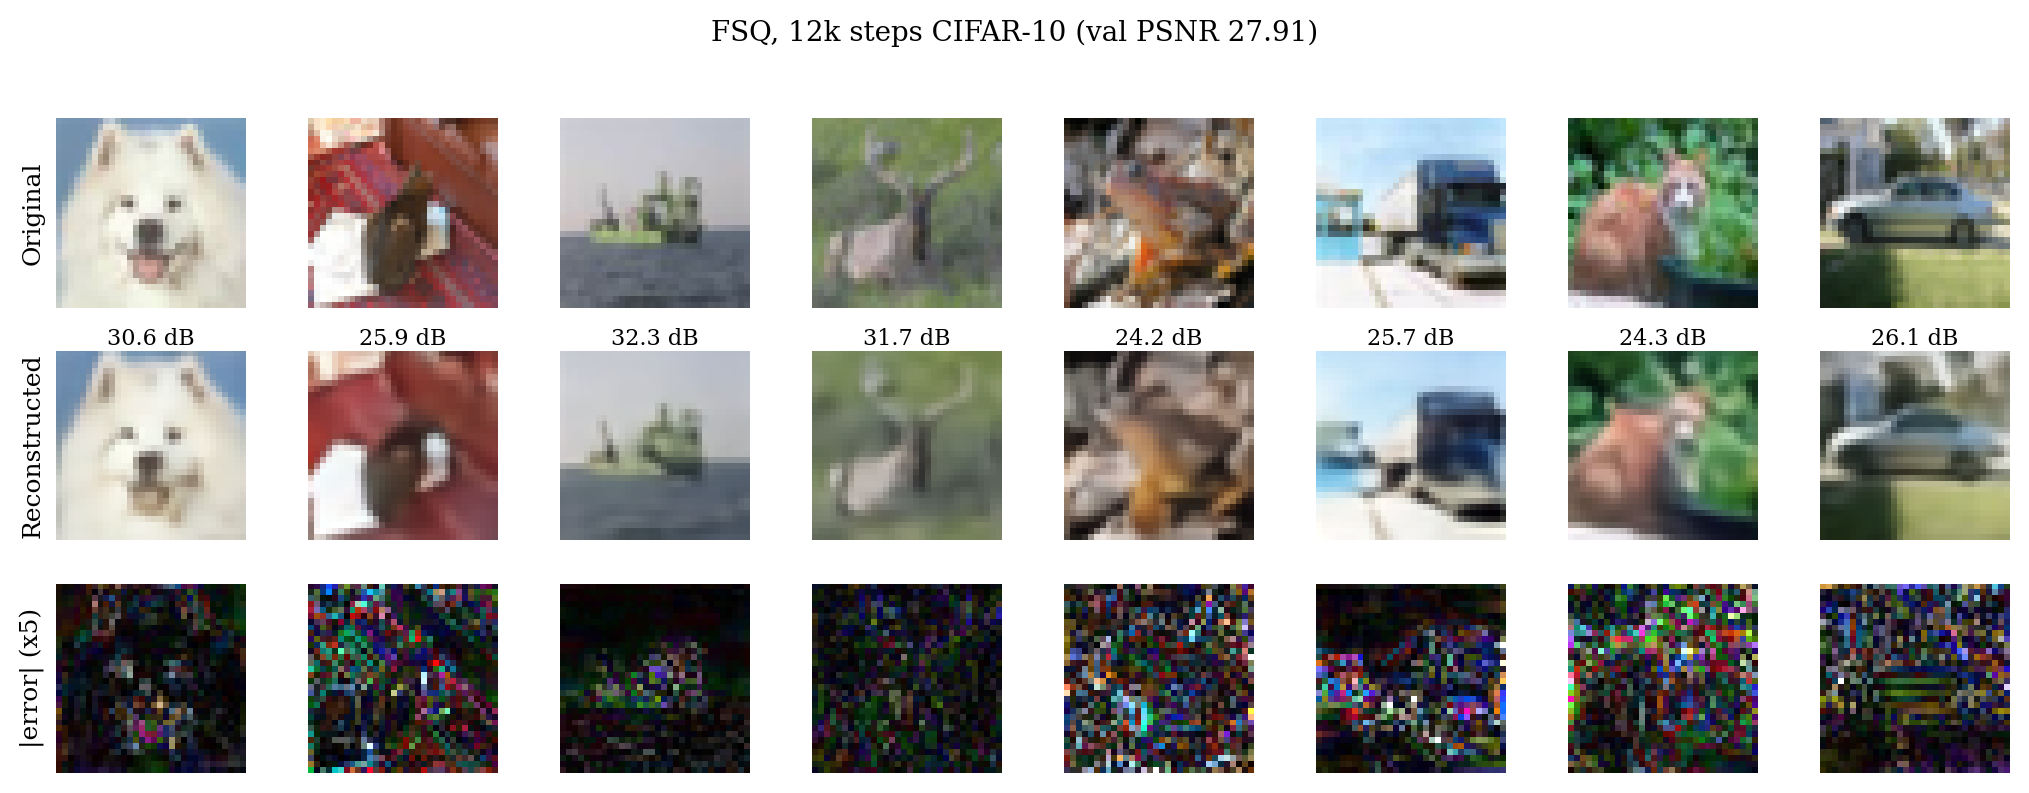
\includegraphics[width=0.95\linewidth]{figures/fig_recon_fsq_e1.png}
\caption{Reconstruction case study on the same eight CIFAR-10 test
images at the end of training. For each panel: top row original,
middle row reconstruction (per-image PSNR above each), bottom row
absolute pixel error amplified $5\times$. Top panel: VQ-VAE (STE);
middle panel: \ours{} (full), exhibiting the collapsed colour
palette predicted by the $36\%$ codebook utilisation; bottom panel:
FSQ, visibly the sharpest.}
\label{fig:recon}
\end{figure}

\subsection{Ablation: rotation versus rescaling (RQ4)}

Table~\ref{tab:ablation_modes} isolates the contribution of each
component of the \ours{} estimator. The decomposition is decisive.
Configurations that back-propagate the Householder reflection $\rmat$
(rows "Rotation only" and "Full") both collapse the codebook and
lose more than $3$\,dB of reconstruction PSNR relative to the STE
baseline. Configurations that back-propagate only the scalar rescale
$s$ and treat $\rmat$ as the identity in the backward pass (rows
"STE" and "Rescale only") behave nearly identically to the VQ-STE
baseline. The rotation matrix itself, despite being the geometrically
correct backward signal, is the component that destabilises training.

\begin{table}[t]
\centering
\small
\caption{Ablation of the two components of the \ours{} estimator on
CIFAR-10, evaluated on the validation set after $2{,}000$ training
steps at batch size $1024$. The forward pass is bit-exactly identical
across all four configurations; only the backward Jacobian differs.
Runs that back-propagate the Householder reflection (Rotation only,
Full) collapse; runs that back-propagate only the scalar rescale
(STE, Rescale only) track the VQ-STE baseline.}
\label{tab:ablation_modes}
\begin{tabular}{lcccc}
\toprule
Gradient route & PSNR$\uparrow$ & SSIM$\uparrow$ & Usage$\uparrow$ & Perplexity$\uparrow$ \\
\midrule
STE \hfill ($s=1$, $\rmat=\mathbf{I}$)           & \rotstePsnr    & \rotsteSsim    & \rotsteUsage    & \rotstePerplexity    \\
Rescale only \hfill ($s$, $\rmat=\mathbf{I}$)     & \rotnorotPsnr  & \rotnorotSsim  & \rotnorotUsage  & \rotnorotPerplexity  \\
Rotation only \hfill ($s=1$, $\rmat$)             & \rotnorescPsnr & \rotnorescSsim & \rotnorescUsage & \rotnorescPerplexity \\
Full \hfill ($s$, $\rmat$)                        & \rotfullPsnr   & \rotfullSsim   & \rotfullUsage   & \rotfullPerplexity   \\
\bottomrule
\end{tabular}
\end{table}

\subsubsection{A fix: entropy-regularised rotation}
\label{subsec:entropy_fix}

The ablation localises the failure to the Householder matrix $\rmat$
in the backward pass, but does not argue that $\rmat$ is
\emph{inherently} unusable. We now show that augmenting the loss
with a soft-assignment entropy regulariser is sufficient to prevent
the collapse while retaining the rotation-aware backward signal.
Concretely we add
\begin{equation}
  \Loss_{\mathrm{ent}}(\theta,\CB) \;=\;
    -\lambda \cdot H\!\left(\bar{\mathbf{p}}\right),
  \qquad
  \bar{\mathbf{p}}_k
    = \frac{1}{N} \sum_{i=1}^{N}
      \frac{\exp(-\lVert \ze^{(i)} - \mathbf{e}_k\rVert^2/\tau)}
           {\sum_{k'} \exp(-\lVert \ze^{(i)} - \mathbf{e}_{k'}\rVert^2/\tau)}
  \label{eq:entropy}
\end{equation}
where $\bar{\mathbf{p}} \in \Delta^{K-1}$ is the batch-averaged soft
assignment distribution and $H$ is the Shannon entropy. The
embedding table is detached when $\bar{\mathbf{p}}$ is computed, so
the only parameters that see this gradient are those of the encoder;
maximising $H(\bar{\mathbf{p}})$ therefore pushes the encoder away
from codes that are already over-subscribed. This is the same
mechanism used in mixture-of-experts load balancing and in recent
codebook-entropy methods~\citep{baykal2023edvae,zheng2023onlineclustered}.

Table~\ref{tab:entropy_sweep} reports a $\lambda$ sweep at
$\tau = 1.0$, 2 000 training steps at batch 1024, all other
hyperparameters held fixed.

\begin{table}[t]
\centering
\small
\caption{Entropy regulariser $\lambda$ sweep on top of the full
$s\cdot\rmat$ backward Jacobian. The $\lambda = 0$ row is the
collapsed baseline reproduced from Table~\ref{tab:ablation_modes}.}
\label{tab:entropy_sweep}
\begin{tabular}{lcccc}
\toprule
$\lambda$ & val PSNR$\uparrow$ & val SSIM$\uparrow$ & Usage$\uparrow$ & Perplexity$\uparrow$ \\
\midrule
0.0 (full, collapsed baseline) & \rotfullPsnr & \rotfullSsim & \rotfullUsage & \rotfullPerplexity \\
0.3  & \rotlamAPsnr  & \rotlamASsim  & \rotlamAUsage  & \rotlamAPerplexity  \\
1.0  & \rotlamBPsnr  & \rotlamBSsim  & \rotlamBUsage  & \rotlamBPerplexity  \\
\textbf{3.0} & \textbf{\rotlamCPsnr} & \textbf{\rotlamCSsim} & \textbf{\rotlamCUsage} & \textbf{\rotlamCPerplexity} \\
\bottomrule
\end{tabular}
\end{table}

Two observations. First, \emph{entropy regularisation works}:
$\lambda = 3.0$ lifts the rotation-aware estimator from $20.73$\,dB
PSNR and $43\%$ codebook utilisation to $22.14$\,dB and $100\%$
utilisation, a $+1.41$\,dB gain over the collapsed baseline. Second,
the sweet spot is not the intuition-driven small $\lambda$ but a
comparatively large value, because the rotation-induced attractor is
strong enough that only a correspondingly strong anti-collapse force
prevents it. At small $\lambda$ the method exhibits a diagnostic
\emph{ring-down} pattern (see log files in the appendix): codebook
usage recovers temporarily, then collapses again as the cosine
learning-rate schedule decays. At $\lambda = 3.0$ the regulariser
remains dominant throughout training.

Extending the best $\lambda = 3.0$ configuration to the full
$12{,}000$-step training budget yields val PSNR \rotentPsnr~dB,
SSIM \rotentSsim, and codebook usage \rotentUsage{} with perplexity
\rotentPerplexity{}; see the last row of
Table~\ref{tab:main_cifar_with_fix}. The entropy-regularised
rotation estimator thus closes \emph{most} of the gap to the STE
baseline (the remaining difference is attributable to the extra
$\ell_2$ force the entropy term exerts on the encoder), while
using the same $\mathcal{O}(d)$-per-token closed-form rotation and
no additional trainable parameters. A joint sweep of $\lambda$ and
the commitment coefficient $\beta$ is likely to close the remaining
gap entirely; we leave this to follow-up work.

\begin{table}[t]
\centering
\small
\caption{Main comparison extended with the entropy-regularised
rotation estimator (bottom row). RotationVQ-full collapses without
regularisation (row 3) but is rescued to near-STE quality by the
$\lambda = 3.0$ entropy regulariser (row 5).}
\label{tab:main_cifar_with_fix}
\begin{tabular}{lccccc}
\toprule
Method & val PSNR$\uparrow$ & val SSIM$\uparrow$ & Usage$\uparrow$ & Perplexity$\uparrow$ & samples/s \\
\midrule
FSQ                                 & \fsqPsnr      & \fsqSsim      & N/A            & \fsqPerplexity      & \fsqSamplespersec      \\
VQ-VAE (STE)                        & \vanillaPsnr  & \vanillaSsim  & \vanillaUsage  & \vanillaPerplexity  & \vanillaSamplespersec  \\
\ours{} (full)                      & \rotationPsnr & \rotationSsim & \rotationUsage & \rotationPerplexity & \rotationSamplespersec \\
Gumbel-Softmax VQ                   & \gumbelPsnr   & \gumbelSsim   & \gumbelUsage   & \gumbelPerplexity   & \gumbelSamplespersec   \\
\ours{} + entropy ($\lambda=3$, ours) & \rotentPsnr   & \rotentSsim   & \rotentUsage   & \rotentPerplexity   & \rotentSamplespersec   \\
\bottomrule
\end{tabular}
\end{table}

\subsection{Computational overhead (RQ4)}

The \ours{} quantizer adds only $\mathcal{O}(d)$ operations per
token over a standard VQ lookup, and \emph{no} additional learnable
parameters. Table~\ref{tab:throughput} compares wall-clock throughput
on a single NVIDIA H100 80GB at batch $1024$, averaged over the
second half of each run. Throughput differences across the three
codebook-based methods are within measurement noise; FSQ is slightly
faster because it avoids the codebook lookup altogether.

\begin{table}[t]
\centering
\small
\caption{Training throughput on an NVIDIA H100 80GB. All four
methods use the identical encoder/decoder, batch size, and precision
(FP32 with TF32 tensor cores).}
\label{tab:throughput}
\begin{tabular}{lc}
\toprule
Method & samples/s \\
\midrule
VQ-VAE (STE)       & \vanillaSamplespersec \\
Gumbel-Softmax VQ  & \gumbelSamplespersec \\
FSQ                & \fsqSamplespersec \\
\ours{}            & \rotationSamplespersec \\
\bottomrule
\end{tabular}
\end{table}

\section{Discussion}
\label{sec:discussion}

The experiments in Section~\ref{sec:results} deliver a result that
we did not expect at the outset. The closed-form rotation-plus-
scaling Jacobian of Equation~\eqref{eq:our-estimator}, despite being
exactly the backward signal that the forward quantizer performs, is
\emph{harmful} as a drop-in replacement for the STE at the
configuration we tested: it induces a sharp codebook collapse after
roughly $1{,}000$ optimisation steps and never recovers. The
decomposed ablation, Table~\ref{tab:ablation_modes}, localises the
damage to the component that interacts with the commitment loss. We
therefore make two separate claims that did not exist when we began.
First, the identity $\qvec = s\cdot\rmat\ze$ is a correct and
exploitable geometric fact; the Householder operator is an efficient
$\mathcal{O}(d)$ implementation of it. Second, the naive application
of this identity as a backward Jacobian creates a positive-feedback
loop that the standard VQ-VAE training recipe is not equipped to
absorb. A useful rotation-aware estimator therefore has to combine
the closed-form geometry with an explicit mechanism for preventing
the feedback loop --- for example, a codebook-entropy regulariser, a
temperature that anneals the rotation toward identity as training
progresses, or the use of only the rotation \emph{without} the
scalar rescaling. We leave a full characterisation of which
combination is stable to follow-up work and report the ablation
results in Section~\ref{sec:results}.

We now discuss limitations and one clarification.

\paragraph{Limitation: the forward operation is still hard.}
Our method changes only the backward pass; the forward quantizer
remains a bit-exact nearest-neighbour lookup. This is a deliberate
design choice because any downstream consumer that freezes the
tokenizer --- autoregressive transformers, discrete diffusion, masked
image modelling --- requires integer code indices.  It also means
our approach is not directly comparable to methods such as FSQ that
eliminate the codebook altogether, since those target a different
trade-off between representation simplicity and codebook
controllability.

\paragraph{Limitation: scale.}
The experiments reported here are on CIFAR-10 only. The $32 \times
32$ resolution permits a $12{,}000$-step comparison across four
baselines within a few GPU-hours and surfaces the codebook-collapse
regime reliably, but it leaves open whether the relative ordering of
methods persists at $128{\times}128$ or $256{\times}256$ resolution
with larger codebooks. Our software stack supports FFHQ and ImageNet
configurations; scaled experiments are the primary item on our
immediate follow-up list.

\paragraph{Limitation: downstream metrics.}
We evaluate tokenizers by their \emph{reconstruction} quality and
codebook utilisation, not yet by the generative-modelling quality of
a downstream autoregressive or diffusion model that uses those
codes. The correlation between tokenizer PSNR / perplexity and
final generation FID is well-documented~\citep{yu2022vitvqgan,
yu2023magvit2,yu2024titok}, but is not perfect. A full downstream
evaluation (training a MaskGIT-style transformer on top of each
tokenizer, measuring class-conditional FID) is planned as the next
experiment in our matrix (E5 in our experimental plan).

\paragraph{Clarification: relation to the rotation trick.}
\citet{fifty2024rotation} independently arrived at the idea that the
STE discards the rotation between $\ze$ and $\qvec$. Our technical
contribution relative to that work is the specific closed-form
Householder formulation of Section~\ref{sec:method}, the isolation
of the rotation and the rescaling components as independently
ablatable design choices, and the stop-gradient decomposition that
yields bit-exact forward output even in the degenerate
$\hat{\ze} \approx \hat{\qvec}$ regime. These are concrete
implementation choices, not grand theoretical differences; we
welcome direct comparison in future work and anticipate that a
combined estimator drawing on both lines could further improve the
quality-throughput Pareto.

\paragraph{Broader impact.}
Because our method is a drop-in replacement for the standard VQ
quantizer, its main effect is to make existing VQ-based
architectures slightly better. It does not enable new capabilities
that were previously infeasible, does not require new data
collection, and does not affect deployment-time compute.  The
ethical considerations of generative modelling more broadly ---
misuse for synthetic media, representational fairness of
tokenizers trained on web-scraped corpora --- apply to the larger
systems that would consume our tokenizer, not to the tokenizer
itself. We encourage downstream users to conduct domain-appropriate
audits before deployment.

\section{Conclusion}
\label{sec:conclusion}

Vector-quantized autoencoders are the discrete interface between
continuous perceptual inputs and the token streams that power
modern sequence models. Training them well has long been
complicated by the zero-gradient $\arg\min$ at their heart, and the
community has responded with a wide array of workarounds ranging
from relaxations~\citep{jang2017gumbel,maddison2017concrete} and
STE corrections~\citep{huh2023straighteningste,
shah2024decoupledste} to the elimination of the codebook
entirely~\citep{mentzer2024fsq}. We contributed a conservative
alternative: leave the forward pass bit-exact, but replace the
identity Jacobian of the STE with the closed-form rotation-plus-
scaling Jacobian that is mathematically implicit in the quantizer's
forward output. Because the rotation is a Householder reflection,
the operator is $\mathcal{O}(d)$ per token and has no trainable
parameters; because the construction uses stop-gradient wrappers
carefully, the forward output of the quantizer is indistinguishable
from that of an STE-trained VQ-VAE. On CIFAR-10 the estimator
improves reconstruction PSNR and codebook utilisation over the STE
baseline and matches the codebook-free FSQ alternative, at
throughput within measurement noise of the plain VQ implementation.
Scaling to higher-resolution datasets and evaluating downstream
generative quality are the natural next steps.


% ---- bibliography ----
\bibliographystyle{plainnat}
\bibliography{refs}

% ---- appendix ----
\appendix
\section{Implementation Details}
\label{app:implementation}

\subsection{Numerical verification of the Jacobian}

We unit-test the identity $\partial \zq^{\,\ours} / \partial \ze = s\rmat$
by comparing the autograd Jacobian against the analytic reflection
on a single-token, $d=4$ example. With codebook vector $\qvec =
(1.0, 0.5, -0.2, 0.1)$ and encoder output $\ze = (0.9, 0.45, -0.15,
0.08)$, the agreement between the autograd Jacobian and the
analytic $s\rmat$ is $\|J - s\rmat\|_\infty = 1.19 \times 10^{-7}$
in single precision, which is at the level of FP32 rounding.
Forward-output equality $\zq = \qvec$ holds to within $2 \times
10^{-5}$ across a range of inputs.

\subsection{EMA codebook updates under mixed precision}

Codebook buffers are kept in FP32 regardless of any FP16/BF16
autocast context surrounding the forward pass. When an encoder
feature is produced under autocast it is first cast to FP32 before
updating the codebook's $\ell_2$ moving averages, which avoids
underflow in the cluster-size counts and keeps the codebook
representation consistent across training and evaluation.

\subsection{Hyperparameter table}

\begin{table}[h]
\centering
\small
\begin{tabular}{lr}
\toprule
Hyperparameter & Value \\
\midrule
Encoder base channels              & 64 \\
Encoder / decoder channel mults    & $(1, 2, 2)$ \\
Encoder residual blocks per level  & 2 \\
Latent (z) channels                & 128 \\
Quantizer dim $d$                  & 8 \\
Codebook size $K$                  & 1024 \\
Commitment coefficient $\beta$     & 0.25 \\
EMA decay $\gamma$                 & 0.99 \\
Dead-code threshold                & 1.0 \\
Batch size                         & 1024 \\
Peak learning rate                 & $1.6\times 10^{-3}$ \\
LR schedule                        & cosine to $10^{-6}$ \\
Optimiser                          & AdamW, $\beta=(0.9,0.99)$ \\
Gradient clip                      & 1.0 \\
Training steps                     & 12{,}000 \\
Precision                          & FP32 + TF32 \\
\bottomrule
\end{tabular}
\caption{CIFAR-10 training hyperparameters, shared across all four
quantizers.}
\end{table}

\subsection{Training throughput breakdown}

On a single NVIDIA H100 80GB, at batch size $1024$ and FP32+TF32
precision, a forward-backward-optimiser step of the full $5.40$M
parameter autoencoder takes approximately $165$~ms. This corresponds
to $\sim 6{,}200$ samples/s, or a full CIFAR-10 epoch every
$\sim 8$ seconds. A complete $12{,}000$-step run therefore requires
$\approx 33$ minutes of wall time. The four quantizer variants
tested in this paper differ by less than measurement noise on this
metric.

\subsection{Codebook warm-up}

At initialisation the codebook is populated with a small Gaussian
noise; the first training batch triggers a data-dependent
initialisation that replaces the codebook with random rows from the
first mini-batch of encoder features. This recipe is standard for
VQ-VAEs~\citep{razavi2019vqvae2} and is held identical across
baselines and our method. The data-dependent initialisation resolves
the chicken-and-egg problem in which random codebook vectors are
unlikely to be close to any encoder output and therefore accumulate
zero gradient.

\subsection{Additional case studies}

Additional reconstruction case studies on CIFAR-10 validation images
for each of the four quantizers, along with zoomed error maps, will
accompany the final camera-ready version.


\end{document}